% Template Oficial da Revista Physicae Organum
%   Equipe Physicae Organum
%-----------------------------

% Vá até a linha com o texto "EDITE A PARTIR DAQUI".
% Você terá que inserir título, autores, instituição, notas, resumo, palavras-chave, textos das seções e bibliografia.
% Para facilitar, colocamos o comentário "[EDITAR]" nas linhas que terão que ser alteradas.
% Indicamos alguns tutorias LaTeX ao final desta página.

% Definição do documento e pacotes utilizados. 

\documentclass[12pt,a4paper,twoside]{article}

% Configurações:

\input{conf/texto.tex}
\input{conf/matematica.tex}
\input{conf/ciencia.tex}
\usepackage{mdframed}
\usepackage{environ} % usado nas definições
\theoremstyle{definition}

% Definição:
\mdfdefinestyle{definitionSty}{backgroundcolor=physorg!10, linewidth=0pt, innerleftmargin=3ex, innerrightmargin=3ex, innertopmargin=1ex, innerbottommargin=1ex, innermargin =0, outermargin =0}
\newcounter{definitionCounter}[section]
%\numberwithin{definitionCounter}{section}
\newmdtheoremenv[style=definitionSty]{definicao}[definitionCounter]{Defini\c{c}\~{a}o}

% Teorema:
\mdfdefinestyle{theoremSty}{backgroundcolor=physorg!10, linewidth=0pt, innerleftmargin=3ex, innerrightmargin=3ex, innertopmargin=1ex, innerbottommargin=1ex, innermargin=0, outermargin=0}
\newcounter{theoremCounter}[section] 
%\numberwithin{theoremCounter}{section}
\newmdtheoremenv[style=theoremSty]{teorema}[theoremCounter]{Teorema}

% Propriedade:
\mdfdefinestyle{theoremSty}{backgroundcolor=physorg!6, linewidth=0pt, innerleftmargin=3ex, innerrightmargin=3ex, innertopmargin=1ex, innerbottommargin=1ex, innermargin=0, outermargin=0}
\newcounter{propertyCounter}[section] 
%\numberwithin{propertyCounter}{section}
\newmdtheoremenv[style=theoremSty]{propriedade}[propertyCounter]{Propriedade}

% Lema
\mdfdefinestyle{lemaSty}{backgroundcolor=physorg!8, linewidth=0pt, innerleftmargin=3ex, innerrightmargin=3ex, innertopmargin=1ex, innerbottommargin=1ex, innermargin=0, outermargin=0}
\newcounter{lemaCounter}[section] 
%\numberwithin{lemaCounter}{section}
\newmdtheoremenv[style=lemaSty]{lema}[lemaCounter]{Lema}

% Demonstração:
\mdfdefinestyle{demonstrationSty}{backgroundcolor=physorg!20, linewidth=0pt, innerleftmargin=3ex, innerrightmargin=3ex, innertopmargin=1ex, innerbottommargin=1ex, innermargin =+1cm, outermargin =+1cm}
\newcounter{demonstrationCounter}[section]
%\numberwithin{demonstrationCounter}{section}
\newmdtheoremenv[style=demonstrationSty]{demonstracao}[demonstrationCounter]{Demonstra\c{c}\~{a}o}

% Axioma:
\mdfdefinestyle{axiomSty}{backgroundcolor=physorg!10, linewidth=0pt, innerleftmargin=3ex, innerrightmargin=3ex, innertopmargin=1ex, innerbottommargin=1ex, innermargin=0, outermargin=0}
\newcounter{axiomCounter}[section] 
%\numberwithin{axiomCounter}{section}
\newmdtheoremenv[style=axiomSty]{axioma}[axiomCounter]{Axioma}

% Exemplo:
\mdfdefinestyle{exampleSty}{backgroundcolor=physorg!10, linewidth=0pt, innerleftmargin=3ex, innerrightmargin=3ex, innertopmargin=1ex, innerbottommargin=1ex,  innermargin =+0.5cm, outermargin =+0.5cm}
\newcounter{exampleCounter}[section]
%\numberwithin{exampleCounter}{section}
\newmdtheoremenv[style=exampleSty]{exemplo}[exampleCounter]{Exemplo}

% Nota:
\mdfdefinestyle{noteSty}{backgroundcolor=physorg!5, linewidth=1pt, innerleftmargin=3ex, innerrightmargin=3ex, innertopmargin=2ex, innerbottommargin=2ex, innermargin =+0.5cm, outermargin =+0.5cm}
\newcounter{noteCounter}[section]
%\numberwithin{noteCounter}{section}
\newmdtheoremenv[style=noteSty]{nota}[noteCounter]{Nota}

% Argumento:
\mdfdefinestyle{argumentSty}{backgroundcolor=physorg!10, linewidth=0pt, innerleftmargin=3ex, innerrightmargin=3ex, innertopmargin=1ex, innerbottommargin=1ex, innermargin=0, outermargin=0} 
\newmdtheoremenv[style=argumentSty]{argumento}{}

% Citação com autor:

\renewenvironment{quotation}
  {\small\list{}{\rightmargin=0.1cm \leftmargin=4cm \topsep=1.5\baselineskip}%
   \item\relax}
  {\endlist}

\def\signed #1{{\leavevmode\unskip\nobreak\newline
  \hbox{}\nobreak #1 %
  \hfil\parfillskip=0pt \finalhyphendemerits=0 \endgraf}}

\newsavebox\mybox
\newenvironment{citacao}[1]
  {\savebox\mybox{#1}\begin{quotation}}
  {\signed{\usebox\mybox}\end{quotation}}

% Para citações:

\usepackage[brazilian,hyperpageref]{backref}
\usepackage[alf,abnt-etal-list=0,abnt-etal-cite=0]{abntex2cite}

% EDITE A PARTIR DAQUI:

\def \tituloportugues {GUIA DE USO DO MODELO DE ARTIGO DA REVISTA PHYSICAE ORGANUM}  % Título. [EDITAR]
\def \tituloingles {USAGE GUIDE OF THE PHYSICAE ORGANUM JOURNAL TEMPLATE}  % Título em inglês. [EDITAR]

% As configurações de layout estão no arquivo mostrado abaixo:
% Para edição da Equipe Physicae Organum:

\setcounter{page}{7} % página inicial do artigo
\def \tipoartigo {Editorial} % pode mudar para "Artigo convidado", "Semana da Física" etc.
\def \tema {\vspace{-1.0em} \small Editoração \vspace{2ex} Científica} % pode mudar para "Artigo convidado", "Semana da Física" etc.
\def \coordenadas {\textit{Physicae Organum}, v. 5, n. 1, p. 7-13, Brasília, 2019.}
\def \paginainternet {http://periodicos.unb.br/index.php/physicae/index}

% Marca d'água:

%\usepackage{draftwatermark}
%\SetWatermarkText{Preprint}
%\SetWatermarkScale{1}
%\SetWatermarkColor[gray]{0.9}

% Pacotes relacionados à parte gráfica do layout:

\usepackage{tikz,everypage}
\usetikzlibrary{calc}
\usetikzlibrary{positioning}
\definecolor{physorg}{RGB}{240,240,226}

\tikzset{%
  line numbers/.store in=\fakelinenos,
  line numbers=45,
  line number shift/.store in=\fakelinenoshift,
  line number shift=0mm,
  line number style/.style={text=gray},
}

% Para abreviar títulos longos no cabeçalho:

\usepackage{truncate}

% Para estilo elegante de cabeçalhos e rodapés:

\usepackage{fancyhdr}
\pagestyle{fancy}

\renewcommand{\headrulewidth}{0pt} % para eliminar linha que separa cabeçalho

\fancyhead[LE]{
\begin{tikzpicture}[overlay, remember picture]%
    \fill[physorg] ($(current page.north west)+(0,-0.5cm)$) rectangle ($(current page.north east)+(0,-1.5cm)$);
    \node[anchor=north west, font=\small, minimum size=1cm, inner xsep=10mm] (PO) at ($(current page.north west)+(0.0cm,-0.5cm)$) {\color{black} \coordenadas};
\end{tikzpicture}
}
\fancyhead[RE]{
}
\fancyhead[LO]{
}
\fancyhead[RO]{
\begin{tikzpicture}[overlay, remember picture]%
    \fill[physorg] ($(current page.north west)+(0,-0.5cm)$) rectangle ($(current page.north east)+(0,-1.5cm)$);
    \node[anchor=north east, font=\small, minimum size=1cm, inner xsep=10mm] (PO) at ($(current page.north east)+(0.0cm,-0.5cm)$) {\truncate{\linewidth}{\tituloportugues}};
\end{tikzpicture}
}


\fancyhead[C]{}
\fancyfoot[C]{}

\fancyfoot[LE]{
\begin{tikzpicture}[overlay, remember picture]%
    \fill[physorg] ($(current page.south west)+(0,0.5cm)$) rectangle ($(current page.south east)+(0,1.5cm)$);
    \node[anchor=south west, text=black, font=\large\scshape, minimum size=.5in] at ($(current page.south west)+(0.5cm,0.4cm)$) {\thepage};
    \node[anchor=south east, text=black, font=\small, minimum size=.5in] at ($(current page.south east)+(-0.5cm,0.4cm)$) {Universidade de Brasília};
\end{tikzpicture}
}
\fancyfoot[RE]{}

\fancyfoot[LO]{}
\fancyfoot[RO]{
\begin{tikzpicture}[overlay, remember picture]%
    \fill[physorg] ($(current page.south west)+(0,0.5cm)$) rectangle ($(current page.south east)+(0,1.5cm)$);
    \node[anchor=south west, text=black, font=\small, minimum size=.5in] at ($(current page.south west)+(0.5cm,0.4cm)$) {Instituto de Física};
    \node[anchor=south east, text=black, font=\large, minimum size=.5in] at ($(current page.south east)+(-0.5cm,0.4cm)$) {\thepage};
\end{tikzpicture}
}

\fancypagestyle{capa}
{

\fancyhead[C]{
\begin{tikzpicture}[overlay, remember picture]%
    \node[anchor=north, font=\small, minimum size=0.8cm, inner xsep=5mm] (titPO) at ($(current page.north)+(0.0cm,-0.1cm)$) {\coordenadas};
    \node[anchor=north, font=\small, minimum size=0.8cm, inner xsep=5mm] (titPO) at ($(current page.north)+(0.0cm,-0.55cm)$) {\color{black} Instituto de Física - Universidade de Brasília};
    \fill[physorg] ($(current page.north west)+(0,-1.5cm)$) rectangle ($(current page.north east)+(-4cm,-2.5cm)$);
    \node[anchor=north west, font=\large\scshape, minimum size=1cm, inner xsep=10mm] (logoPO) at ($(current page.north west)+(0.0cm,-0.5cm)$) {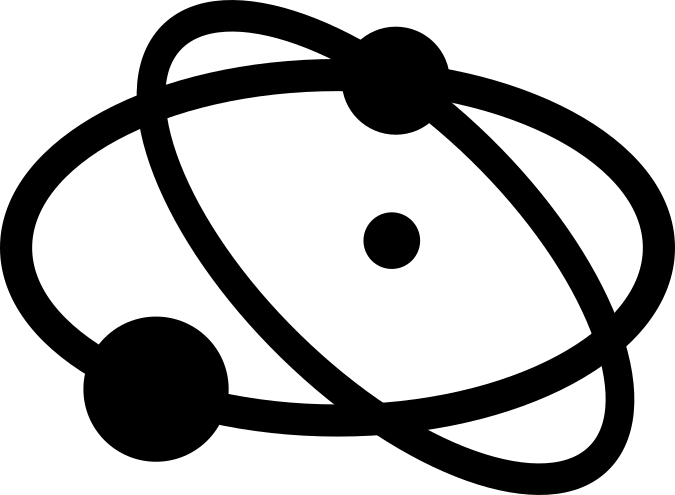
\includegraphics[width=2.0cm]{figs/logo-physicae-organum.png}};
    \node[anchor=north west, font=\large\scshape, minimum size=0.8cm, inner xsep=5mm] (titPO) at ($(current page.north west)+(2.75cm,-1.55cm)$) {\color{black} PHYSIC{\AE} ORGANUM};
    \node[anchor=south east, font=\large\scshape, minimum size=0.8cm, inner xsep=5mm] (secao) at ($(current page.north east)+(-4cm,-2.4cm)$) {\large \tipoartigo};
    \fill[physorg]  ($(current page.north east)+(-3.5cm,-0.5cm)$) rectangle ($(current page.north east)+(-0.5cm,-2.5cm)$);
    \node[text width=2.5cm, anchor=north west, font=\large\scshape, minimum size=0.8cm, inner xsep=5mm] (secao) at ($(current page.north east)+(-3.6cm,-0.8cm)$) {\begin{center} \color{black} \tema \end{center}};
\end{tikzpicture}
}

\fancyhead[EL,OR]{}
\fancyhead[ER]{}
\fancyhead[OL]{}

\fancyfoot[C]{
\begin{tikzpicture}[overlay, remember picture]%
    \fill[physorg] ($(current page.south west)+(0,0.5cm)$) rectangle ($(current page.south east)+(0,1.5cm)$);
    \node[anchor=south west, text=black, font=\small, minimum size=.5in] at ($(current page.south west)+(0.5cm,0.4cm)$) {\href{\paginainternet}{\paginainternet}};
    \node[anchor=south east, text=black, font=\large, minimum size=.5in] at ($(current page.south east)+(-0.5cm,0.4cm)$) {\thepage};
\end{tikzpicture}
}

\fancyfoot[R]{}
\fancyfoot[L]{}

} % Não mexa nesta linha!

% Coloque abaixo os nomes dos autores e o número de suas instituições:

\author[1]{Leonardo Luiz e Castro\thanks{llcastro@unb.br}}
%\author[2]{Coloque aqui outro autor}
%\author[1]{Coloque aqui outro autor}
%\author[2]{Coloque aqui outro autor}
%\author[1]{Coloque aqui outro autor}

% Coloque abaixo os números e nomes das instituições:

\affil[1]{Instituto de Física -- Universidade de Brasília}
%\affil[2]{Coloque aqui outra instituição}
%\affil[3]{Coloque aqui outra instituição}

% Ajustes diversos antes de começar o documento (últimos preparativos),
% tais como atribuição da variável "title", configurações para resolver erros de compilação etc.

\renewcommand\Authsep{, \quad }
\renewcommand\Authand{, }
\renewcommand\Authands{, \quad }

\renewcommand*{\Affilfont}{\normalsize\normalfont}
\renewcommand*{\Authfont}{\scshape}

\title{%
    \vspace{-15mm}%
    \fontsize{20pt}{26pt}%
    \selectfont\textbf{\tituloportugues} \\
    \vspace{1ex}
    \fontsize{14pt}{20pt}\selectfont\textbf{\color{gray}\tituloingles}%
} % Título.
\date{}


% Trecho para evitar conflito entre pacotes Verbatim e TikZ (https://tex.stackexchange.com/questions/352297/tikz-error-some-package-has-redefined-the-meaning-of-the-math-mode-dollar-sign):

\usepackage{everypage}

\makeatletter
\AtBeginDocument{%
  \AddEverypageHook{%
    \small    
    \catcodetable  \catcodetable@latex
  }%
}
\makeatother

%-----------------------------

% Aqui damos início ao documento.

\begin{document}

\maketitle

\thispagestyle{capa}

% Resumo e palavras-chave. 

\hrule

\selectlanguage{portuges}
\begin{abstract}
\noindent
A revista Physicae Organum apresenta um novo modelo para o leiaute de seus artigos, disponível em \LaTeX na Galeria Overleaf.
Explicamos aqui a estrutura básica dos artigos do projeto e os procedimentos para inserção de texto, figuras, tabelas, ambientes diversos (teoremas, axiomas, notas etc.) e referências bibliográficas.
\vspace{\baselineskip} \\
\palavraschave{Física. Modelo de artigo. Editoração. Template. Guia.}
\end{abstract}
\vspace{5mm}

\hrule

\selectlanguage{english}
\begin{abstract}
\noindent
The Physicae Organum journal introduces a new template for its articles, available in \LaTeX in the Overleaf Gallery. 
We explain here the basic structure of the articles of the project and the procedures for insertion of text, figures, tables and diverse environments (theorems, axioms, notes, etc.) and bibliographical references.
\vspace{\baselineskip} \\
\keywords{Physics. History. University. Models of university.}
\end{abstract}
\vspace{5mm}

\hrule

\selectlanguage{portuges}


\section{Introdução}

Physicae Organum é uma revista do Instituto de Física da Universidade de Brasília \cite{physicaeorganum}. Para facilitar a escrita de seu trabalho na Physicae Organum, apresentamos o novo modelo para editoração e diagramação para a revista. Embora a revista aceite submissão de artigos em outros formatos, a diagramação será feita em \LaTeX.

O pessoal das ciências naturais gosta de usar \LaTeX porque essa ferramenta possibilita escrever facilmente equações como
\begin{equation}
 p+\frac{1}{2}{\rho}v^2+{\rho}gh = \text{constante}
 \label{eq:Bernoulli}
\end{equation}
na qual $p$ é a pressão, $v$ é a velocidade e $h$ é a elevação, ou seja, a “altura do tubo”. Essa equação pode ser deduzida a partir do \textit{Teorema Trabalho-Energia}.

\section{Estrutura dos arquivos}

Um projeto \LaTeX consiste de um arquivo principal de extensão \verb|tex| com outros arquivos e (talvez) pastas auxiliares. Esses arquivos e pastas devem estar no mesmo projeto do Overleaf (ou outra plataforma online). Em caso de edição em computador pessoal, os arquivos e pastas do projeto devem estar na mesma localização do sistema de arquivos de seu computador e devem ser compilados com algum programa específico, como o Texmaker ou MikTeX. Ao editar diretamente no sistema Overleaf, todos os pacotes adicionais estarão instalados previamente. No entanto, ao compilar localmente, eles terão que ser instalados no computador. Em Ubuntu Linux, por exemplo, o pacote \verb|texlive-full| instala todos os pacotes necessários (e vários outros). No Windows, pode-se usar o instalador de pacotes adicionais do próprio MikTeX.

O projeto do novo modelo \LaTeX é organizado da seguinte forma:

\begin{itemize}
    \item \verb|main.tex|: arquivo principal com o código \LaTeX;
    \item \verb|main.bib|: arquivo com referências bibliográficas no formato BibTeX;
    \item \verb|logo-physicae-organum.png|: imagem com a logomarca da revista;
    \item \verb|conf|: pasta com código adicional de configuração, sobretudo chamada e configuração de pacotes.
\end{itemize}


\section{Inserindo seu texto}

O primeiro passo é colocar o título de seu artigo, em português e em inglês, substituindo o trecho em maiúsculas na parte do código que aparece assim:

\begin{verbatim}
\def \tituloportugues {COLOQUE SEU TÍTULO EM PORTUGUÊS AQUI}  % Título. [EDITAR]
\def \tituloingles {COLOQUE O TÍTULO EM INGLÊS AQUI}  % Título em inglês. [EDITAR]
\end{verbatim}

Em seguida, você substituirá o texto ``Coloque aqui o texto do seu resumo'' por, adivinhe, pelo texto do resumo de seu artigo! Substitua também as palavras que estão dentro das chaves do comando \verb|\palavraschave{...}| pelas palavras chaves do seu artigo.
\begin{verbatim}
\selectlanguage{portuges}
\begin{abstract}
\noindent
Coloque aqui o texto do seu resumo. % [EDITAR] %
\vspace{\baselineskip} \\
\palavraschave{física, história, universidade, modelos de universidade.}
\end{abstract}
\end{verbatim}
Logo abaixo desse código, há outro semelhante para inserir o resumo e as palavras-chave (\textit{keywords}) em inglês.

Em seguida, inclua os nomes das seções dos seus artigos nos comandos \verb|\section{...}|.

\section{Inserindo figuras e tabelas}

Figuras podem ser inseridas normalmente através do comando \verb|includegraphics|, após serem enviadas ao seu projeto (para edição online) ou guardadas na mesma pasta que o seu arquivo \verb|main.tex|. Por uma questão de organização, você também pode guardar todas as figuras de seu projeto numa subpasta. Por exemplo, para inserir a figura \verb|logo-physicae-organum.png| da pasta \verb|figs|, você pode usar o seguinte código:
\begin{verbatim}
\begin{figure}
    \begin{minipage}{0.5\hsize}
        \centering
        \caption{Logotipo da revista Physicae Organum.}
        \label{fig:logo}
        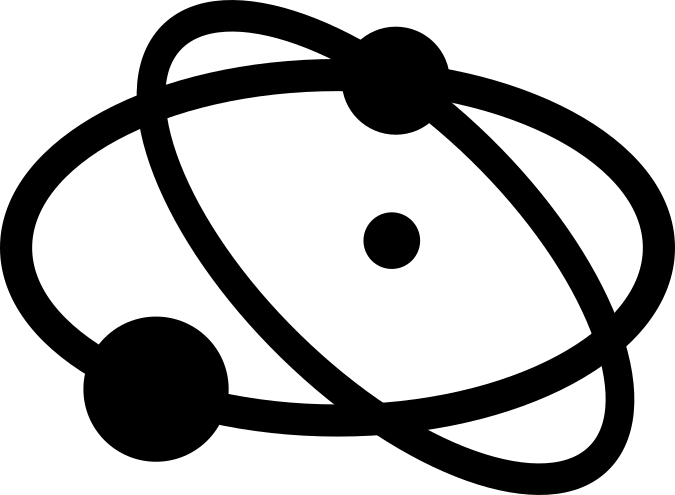
\includegraphics[width=\linewidth]{figs/logo-physicae-organum.png}
        \source{criação de Olavo Leopoldino da Silva Filho.}
    \end{minipage}
\end{figure}
\end{verbatim}

O comando \verb|\centering| centraliza a figura, o ambiente \verb|minipage| serve para definir a largura (\verb|0.5\hsize| significa metade da linha) e fazer com que figura e legenda fiquem alinhadas, \verb|\caption{...}| insere uma legenda, \verb|\label{...}| (que deve vir depois da linha de ``caption'') insere um rótulo para citar a figura no texto com \verb|\ref{...}|, e \verb|\source{...}| informa a fonte da figura. A figura~\ref{fig:logo} mostra o resultado.
\begin{figure}
    \centering
    \begin{minipage}{0.5\hsize}
        \caption{Logotipo da revista Physicae Organum.}
        \label{fig:logo}
        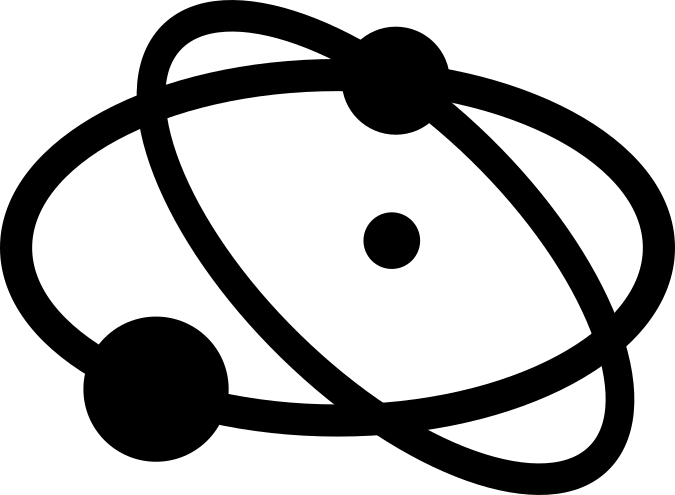
\includegraphics[width=\linewidth]{figs/logo-physicae-organum.png}
        \source{criação de Olavo Leopoldino da Silva Filho.}
    \end{minipage}
\end{figure}


Tabelas podem ser inseridas de forma semelhante:
\begin{verbatim}
\begin{table}
\begin{minipage}{\hsize}
\begin{center}
	\caption{Algumas unidades básicas do SI.}
	\label{tab:SI-basicas}
	\begin{tabular}{P{0.40\hsize}|P{0.5\hsize}}
		\hline
		\textbf{Grandeza} & \textbf{Unidade} \\
		\hline
		comprimento & metro (\si{\meter}) \\
		\hline
		massa & quilograma (\si{\kilo\gram}) \\
		\hline
		tempo & segundo (\si{\second}) \\
		\hline
		corrente elétrica & ampère (\si{\ampere}) \\
		\hline
		temperatura & kelvin (\si{\kelvin}) \\
		\hline
		quantidade de matéria & mol (\si{\mol}) \\
		\hline
		intensidade luminosa & candela (\si{\candela}) \\
		\hline
	\end{tabular}
	\source{adaptado do livro Física para Ciências Agrárias e Ambientais,
	de Leonardo Luiz e Castro e Olavo Leopoldino da Silva Filho \cite{Castro-2019}.}
\end{center}
\end{minipage}
\end{table}
\end{verbatim}
A tabela~\ref{tab:SI-basicas} mostra o resultado.

\clearpage % Este comando descarrega todos os comandos acima e passa para a próxima página.

\begin{table}
    \centering
    \begin{minipage}{0.5\hsize}
    	\caption{Algumas unidades básicas do SI.}
	    \label{tab:SI-basicas}
	    \begin{tabular}{c|c}
		    \hline
		    \textbf{Grandeza} & \textbf{Unidade} \\
		    \hline
		    comprimento & metro (\si{\meter}) \\
		    \hline
		    massa & quilograma (\si{\kilo\gram}) \\
		    \hline
		    tempo & segundo (\si{\second}) \\
		    \hline
		    corrente elétrica & ampère (\si{\ampere}) \\
		    \hline
		    temperatura & kelvin (\si{\kelvin}) \\
		    \hline
		    quantidade de matéria & mol (\si{\mol}) \\
		    \hline
		    intensidade luminosa & candela (\si{\candela}) \\
		    \hline
	    \end{tabular}
	    \source{adaptado do livro Física para Ciências Agrárias e Ambientais, de Leonardo Luiz e Castro e Olavo Leopoldino da Silva Filho.}
    \end{minipage}
\end{table}

\section{Ambientes e bibliografia}

No arquivo \verb|ambientes.tex|, que está na pasta \verb|conf|, encontram-se definições de ambientes (tipos de caixas de texto) que são numeradas automaticamente. Por exemplo, o código abaixo gera uma caixa ``Definição 1''.
\begin{verbatim}
\begin{definicao}
    Physicae Organum: revista do Instituto de Física.
\end{definicao}
\end{verbatim}
Fica assim:
\begin{definicao}
    Physicae Organum: revista do Instituto de Física.
\end{definicao}
Uma outra definição receberá o número seguinte:
\begin{definicao}
    Instituto de Física: instituto da Universidade de Brasília no qual se estuda física.
\end{definicao}

De forma análoga, você pode criar os ambientes ``teorema'', ``demonstração'', ``axioma'', ``lema'', ``nota'', ``argumento'', ``definição'' e ``exemplo''. Nos comandos, não use acentuação; uma demonstração, por exemplo, deve ser definida assim:
\begin{verbatim}
\begin{demonstracao}
    Isto deveria ser uma demonstração.
\end{demonstracao}
\end{verbatim}
O resultado é este:
\begin{demonstracao}
    Isto deveria ser uma demonstração.
\end{demonstracao}

Para a bibliografia, recomendamos usar \verb|BibTeX|. Para isso, insira suas referências no formato adequado no arquivo \verb|main.bib|, que já contém vários exemplos de diversos tipos de entrada. A entrada mostrada abaixo insere na base de referências um artigo que chama de \verb|greenwade93|. Esse rótulo é de livre escolha e deve ser usado para citar a referência do texto com o comando \verb|\cite{greenwade93}|. Ao usar esse comando, a citação aparecerá como \cite{greenwade93} e será listada na parte das referências automaticamente.
\begin{verbatim}
@article{greenwade93,
    author  = "George D. Greenwade",
    title   = "The {C}omprehensive {T}ex {A}rchive {N}etwork ({CTAN})",
    year    = "1993",
    journal = "TUGBoat",
    volume  = "14",
    number  = "3",
    pages   = "342--351"
}
\end{verbatim}
Os campos podem vir entre aspas ou entre chaves. Múltiplos autores sempre devem estar separados por \verb|AND| e não por vírgula (o compilador \LaTeX ajustará as referências ao padrão). As vírgulas, por outro lado, podem ser usadas para separar mais claramente a parte do nome completo que deve aparecer como sobrenome. Por exemplo, suponha que você queira citar um artigo escrito por (nomes fictícios) Luís Carlos Costa e Silva, Maria Joaquina da Silva,  Cléber Azevedo Júnior, e José Marcelo de Sousa Carneiro. Poderia entrar com essa referência no arquivo \verb|main.bib| desta forma:
\begin{verbatim}
@article{costaesilva-2017,
    author  = {Costa e Silva, Luís Carlos AND da Silva, Maria Joaquina
                AND Azevedo J\'unior, Cléber AND Carneiro, José Marcelo de Sousa},
    title   = {Este é o nome do nosso artigo!},
    year    = {2017},
    journal = {Revista de Algum Tema Qualquer},
    volume  = {1},
    number  = {3},
    pages   = {42--51}
}
\end{verbatim}
Ao citá-la com \verb|\cite{costaesilva-2017}|, a citação apareceria assim: \cite{costaesilva-2017} (veja como sai na lista de referências).
No início do código, você pode encontrar a linha \verb|\usepackage[alf,abnt-etal-list=0,abnt-etal-cite=3]{abntex2cite}|.
O valor de \verb|abnt-etal-cite| está definido como $3$, o que significa que uma citação será abreviada se tiver três ou mais autores.
O valor de \verb|abnt-etal-list| está definido como $0$, o que significa que a lista de autores nunca será abreviada na lista de referências.

Citações diretas podem ser feitas com o ambiente \verb|citacao|. Veja o exemplo a seguir:
\begin{verbatim}
\begin{citacao}{Carl Sagan}
    Alegações extraordinárias exigem evidências extraordinárias.
\end{citacao}
\end{verbatim}
Esse código gera uma citação assim:
\begin{citacao}{Carl Sagan}
    Alegações extraordinárias exigem evidências extraordinárias.
\end{citacao}
O comando \verb|\cite{...}| pode ser usado como indicação do autor:
\begin{verbatim}
\begin{citacao}{\cite{greenwade93}}
TEX is a typesetting program designed for high-quality composition of material that contains a lot of mathematical and technical expressions. It has been adopted by many authors and publishers who generate technical books and papers. It was created by Professor Donald E. Knuth of Stanford University, originally for preparation of his book series ``The Art of Computer Programming''. TEX has been made freely available by Knuth.
\end{citacao}
\end{verbatim}
Naturalmente, a referência \verb|grennwade93| deve estar definida no arquivo BibTeX (aqui, \verb|main.bib|). Confira o resultado:
\begin{citacao}{\cite{greenwade93}}
TEX is a typesetting program designed for high-quality composition of material that contains a lot of mathematical and technical expressions. It has been adopted by many authors and publishers who generate technical books and papers. It was created by Professor Donald E. Knuth of Stanford University, originally for preparation of his book series ``The Art of Computer Programming''. TEX has been made freely available by Knuth.
\end{citacao}

\section{Pacotes científicos}

Existem muitos pacotes \LaTeX voltados à ciência. Recomendamos fortemente que você aprenda a usar \textit{SIunits} para escrever grandezas no sistema SI com formatação que se ajusta aos padrões do idioma do documento, como \SI{1.23e-4}{\meter\per\second}.
Você também pode usar pacotes como o \verb|mhchem| para escrever fórmulas químicas como \ce{H2O}, \ce{^{227}_{90}Th+} ou \cite{moodle-mhchem}
\begin{equation}
    K = \frac{[\ce{Hg^2+}][\ce{Hg}]}{[\ce{Hg2^2+}]}.
    \label{eq:chem}
\end{equation}
Você pode até mesmo fazer gráficos e figuras científicas diretamente no código \LaTeX, usando pacotes como \textit{PGFPlots}, \textit{PSTricks}, \textit{Metapost} e \textit{Tikz}. Pesquise galerias de imagens feitas com esses pacotes!

\section{Agradecimentos}

A Olavo Leopoldino da Silva Filho, Marcello Ferreira e Fábio Luís de Oliveira Paula, pela ajuada no desenvolvimento do template original, a partir do qual este guia foi feito.

\bibliography{main}

\end{document}

% Tutoriais LaTeX:

% <http://www.mat.ufmg.br/~regi/topicos/intlat.pdf>
% <http://ece.uprm.edu/~caceros/latex/introduction.pdf>

%-----------------------------

% LaTeX Online (free account):

% <https://www.overleaf.com/>

%-----------------------------

% Códigos matemáticos LaTeX:

% <http://www.codecogs.com/latex/eqneditor.php>

%-----------------------------

% Construir tabelas no LaTeX:

% <http://www.tablesgenerator.com/#>

%-----------------------------